\documentclass[11pt]{article}
\usepackage[utf8]{inputenc}
\usepackage{amsfonts}
\usepackage{natbib}
\usepackage{graphicx}
\usepackage{amsmath}
\usepackage{amssymb}
\usepackage{mathrsfs} % Cursive font
\usepackage{graphicx}
\usepackage{ragged2e}
\usepackage{fancyhdr}
\usepackage{nameref}
\usepackage{wrapfig}




\usepackage{mathtools}
\usepackage{xparse} \DeclarePairedDelimiterX{\Iintv}[1]{\llbracket}{\rrbracket}{\iintvargs{#1}}
\NewDocumentCommand{\iintvargs}{>{\SplitArgument{1}{,}}m}
{\iintvargsaux#1}
\NewDocumentCommand{\iintvargsaux}{mm} {#1\mkern1.5mu,\mkern1.5mu#2}

\makeatletter
\newcommand*{\currentname}{\@currentlabelname}
\makeatother

\usepackage[a4paper,hmargin=1in, vmargin=1.4in,footskip=0.25in]{geometry}


%\addtolength{\hoffset}{-1cm}
%\addtolength{\hoffset}{-2.5cm}
%\addtolength{\voffset}{-2.5cm}
\addtolength{\textwidth}{0.2cm}
%\addtolength{\textheight}{2cm}
\setlength{\parskip}{8pt}
\setlength{\parindent}{0.5cm}
\linespread{1.5}

\pagestyle{fancy}
\fancyhf{}
\rhead{TP1}
\lhead{Teoría de Bases de Datos}
\rfoot{\vspace{1cm} \thepage}

\renewcommand*\contentsname{\LARGE Índice}

\begin{document}

\begin{titlepage}
    \begin{center}
        \vfill
        \vfill
            \vspace{0.7cm}
            \noindent\textbf{\Huge Trabajo Práctico 1}\par
            \noindent\textbf{\Huge Teoría de Bases de Datos}\par
            \vspace{.5cm}
        \vfill
        \noindent \textbf{\huge Integrantes:}\par
        \vspace{.5cm}

        \noindent \textbf{\Large Bisiach, Ezequiel (B-6199/9)}\par
        \noindent \textbf{\Large Cipullo, Inés (C-6867/5)}\par
        \noindent \textbf{\Large Sullivan, Katherine (S-5436/4)}\par
 
        \vfill
        \large Universidad Nacional de Rosario \par
        \noindent\large 2021
    \end{center}
\end{titlepage}
\ \par


\section*{Diagrama Entidad-Relación}

\hspace{-1.5cm}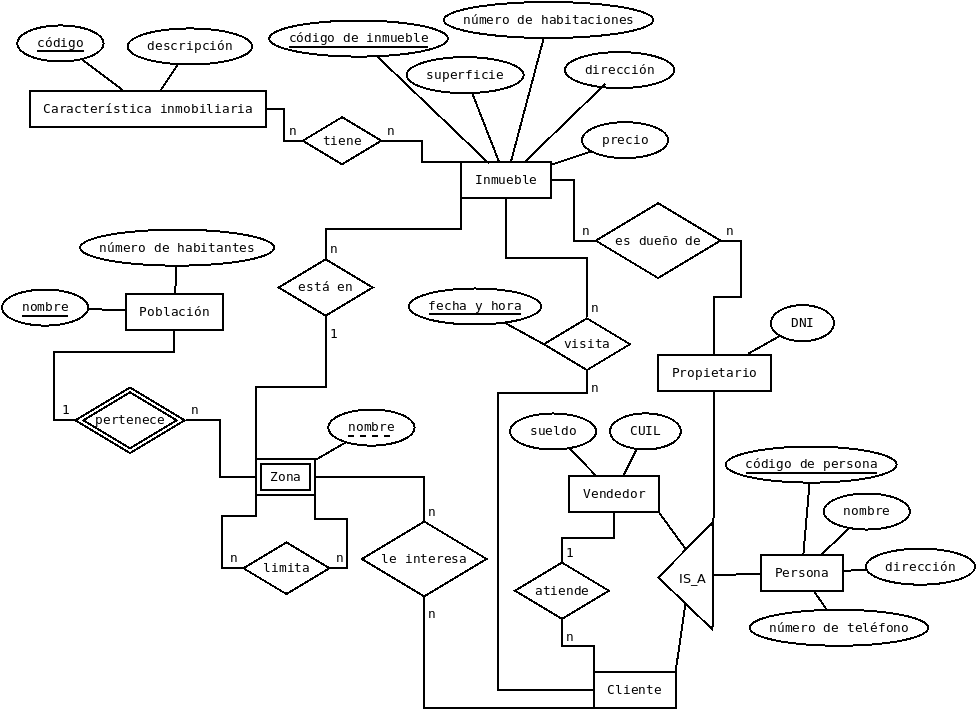
\includegraphics[scale=.55]{../Diagrama1.png}


\section*{Observaciones}

\begin{itemize}
    \item Nos resulto adecuado utilizar la estructura IS\_A para generalizar la entidad Persona y así nuclear todos los atributos en común de las entidades Propietario, Cliente y Vendedor.
    \item En la relación Visita, la fecha y la hora forman un único atributo y este es clave ya que nos interesa mantener un registro de todas las visitas que fueron realizadas.
\end{itemize}


\end{document}